% ********** Rozdział 2 **********
\chapter{Tytuł rozdziału}


\section{Struktura projektu}
\begin{figure}[!ht]
	\centering
		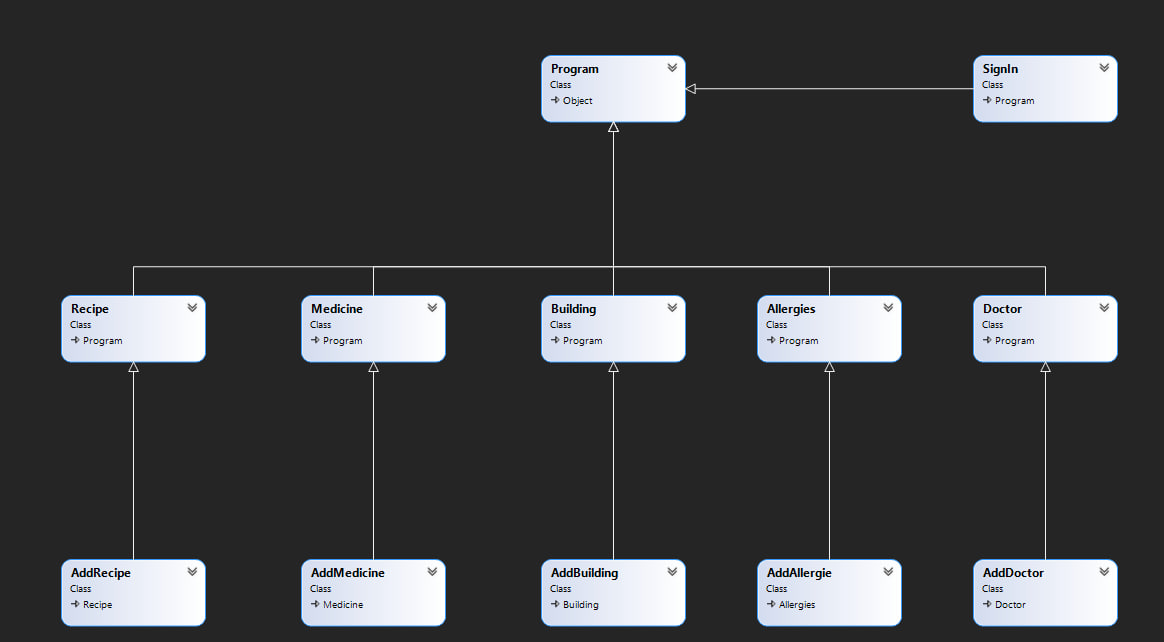
\includegraphics[width=16cm]{diagram.jpg}
	\caption{\footnotesize Diagram klasy z aplikacji}
	\label{fig:plotend}
\end{figure}
Na screenie jest widoczna budowa i połączenia pomiędzy klasami. Program służy jako wspólna baza do wszystkich danych, z których korzysta aplikacja. SignIn - do logowania; Recipe - do zachowania informacji o dostępnych receptach; Medicine - pula informacji o lekach; Building - dane o szpitalach, aptekach oraz przychodniach; Allergies - o alergiach i dt. lekach; Doctor - informacje o lekarzach rodzinnych.

\newpage
\subsection{Opis techniczny}
\begin{figure}[!ht]
	\centering
		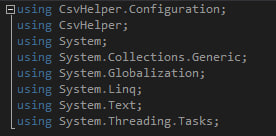
\includegraphics[width=10cm]{labs.jpg}
	\caption{\footnotesize Używane biblioteki}
	\label{fig:plotend}
\end{figure}
Na screenie widoczne są wszystkie użyte biblioteki: - CsvHelper, CsvHelper.Configuration - biblioteki dla pracy z bazą danych na CSV plikach. - Oraz w projekcie importowana biblioteka do pracy z kolekcjami(System.Collections.Generic). System zestaw podstawowch funkcji w języku C#
Zgodnie z wymaganiami projektu, realizowany jest w języku C#
\subsection{Minimalne wymagania sprzętowe}
\begin{itemize}
    \item Processor - Intel Core 2 Duo E8400
    \item Pamięć operacyjna 500 mb
    \item Potęga karty graficznej 524 mb
    \item Miejsce na dysku twardym 100 mb
\end{itemize}
% ********** Koniec rozdziału **********
